\section{Convolutional Neural Network} \label{sec:cnn}
\acrshort{cnn} is a type of \acrshort{nn} specialized in analyzing visual imagery and natural language processing. \acrshort{cnn}s are feedforward, sparsely connected \acrshort{nn}s, and structured as a pipeline of layers \cite{abdelouahab_accelerating_2018}. It has shown superior performances on different competitions related to Computer Vision and Image Processing \cite{khan_survey_2020}. Nowadays, \acrshort{cnn}s are used in character and gesture recognition, video classification, face detection, etc \cite{shawahna_fpga-based_2019}. This section aims at investigating the different aspects of a \acrshort{cnn}.
%Mand the optimizations that could be made to reduce its size and computational complexity.

First, the building blocks of a CNN are developed in the section \ref{subsec:layer} starting from its basic element \textit{the perceptron}. Then, we describe how to use it to build layers which can perform complex functions. Finally, we detail the other types of layers required to improve the efficiency of the model, such as pooling layer.

Then, section \ref{subsec:models} describes how to effectively combine these layers with a focus on state-of-art networks like AlexNet, VGG16, ResNet, and MobileNetV2.

Finally, Section \ref{subsec:train} focuses on the training of a \acrshort{cnn}. We briefly explain the back-propagation algorithm, which consists of a forward-propagation and a back-propagation.
%
%
\subsection{Structure of a CNN} \label{subsec:layer}
%
A CNN is a pipeline of layers which can be stacked to form a network \cite{abdelouahab_accelerating_2018}. A layer is a high-level building block, which consists of a set of operations, weights, and non-linear functions. The output of one layer can be used as input of the next layer or as the final output of the network. 

This section first introduces the simplest building element of a \acrshort{cnn}: the perceptron. We describe its different components and notably its activation function. Then, we can use this element to build more complex layers such as fully connected and convolutional layer. Finally, we present the pooling layer which it used to reduce the spatial dimensions of the ouput of the previous layer.
%
%
\subsection{Perceptron} \label{subs:perceptron}
The perceptron was first developed in 1957 by \textcite{brain_perceptron_nodate}. It is a computational model based on on the brain. The human brain has a huge number of computing units, \textbf{neurons}. A biological neuron receives information (collects charges) from synapses through chemical mechanisms and once a threshold is passed, the cumulate charges are released (we say the neuro fires) and the information is transmitted to other neurons.

Mathematically, a perceptron has n inputs ($x_1$, ..., $x_n$) which can be expressed as vector \textbf{$\bar{x}$}, n wheights (\textbf{$\bar{w}$}) and a bias \textbf{b}. The perceptron, when receiving an input vector, performs a weighted sum. If the wheighted sum is above a threshold (controlled by the bias which can lower or raise it), the perceptron is 'activated' and outputs a non-zero value (1). The figure \ref{fig:perceptron} illustrates this. We can write the operation in a vector form:
%
$$
h(x| w, b) = h(\sum^{n}_{i=1} x_i \cdot w_i + b) = h ( \textbf{$\bar{w}$}^{T} \textbf{$\bar{x}$} + b)
$$
%
where $h$ is the activation function of the perceptron (the section \ref{subs:acti} describes other activation functions)
$$
h ( \textbf{$\bar{w}$}^{T} \textbf{$\bar{x}$} + b) = \begin{cases} 1, & \mbox{if } \textbf{$\bar{w}$}^{T} \textbf{$\bar{x}$} + b > 0 \\ 0, & \mbox{Otherwise} \end{cases}
$$
In the following section \ref{subs:fcl}, we discover how we can use mutliple perceptrons to create a \textbf{fully-connected layer}.
%
\begin{figure}
    \centering
    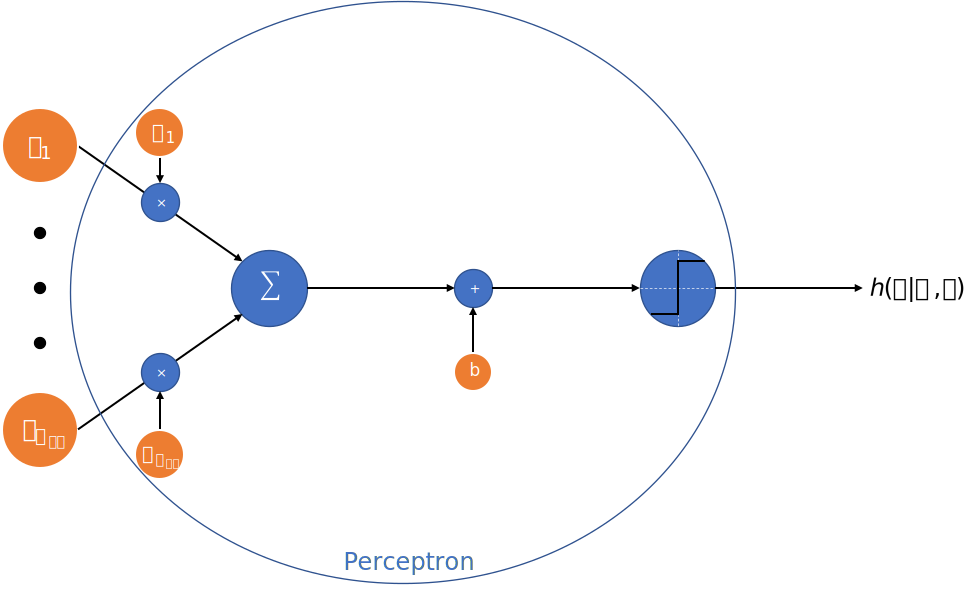
\includegraphics[width=\textwidth]{perceptron.pdf}
    \caption{The Perceptron}
    \label{fig:perceptron}
\end{figure}

%
\subsection{Activation} \label{subs:acti}
The activation function is the non-linear output of the neuron. Its purpose is to decide whether the neuron fires or not. To apply the back-propagation algorithm (see Section \ref{sec:train}), which makes the network learn, we need to have the activation function to be differentiable \cite{lecun_backpropagation_1989}. To optimize the network, we must compute the gradient of the activation function. As the step function described in equation \eqref{eq:step} has a gradient of zero, the perceptron can not learn if we use this activation function. Various activation functions have then been proposed with different properties, as illustrated in Figure \ref{fig:acti}. According to \textcite{khan_survey_2020}, the choice of an appropriate activation function can accelerate the learning phase and some activations have less computational complexity \cite{krizhevsky_imagenet_2012}.
%
\begin{figure}
    \centering
    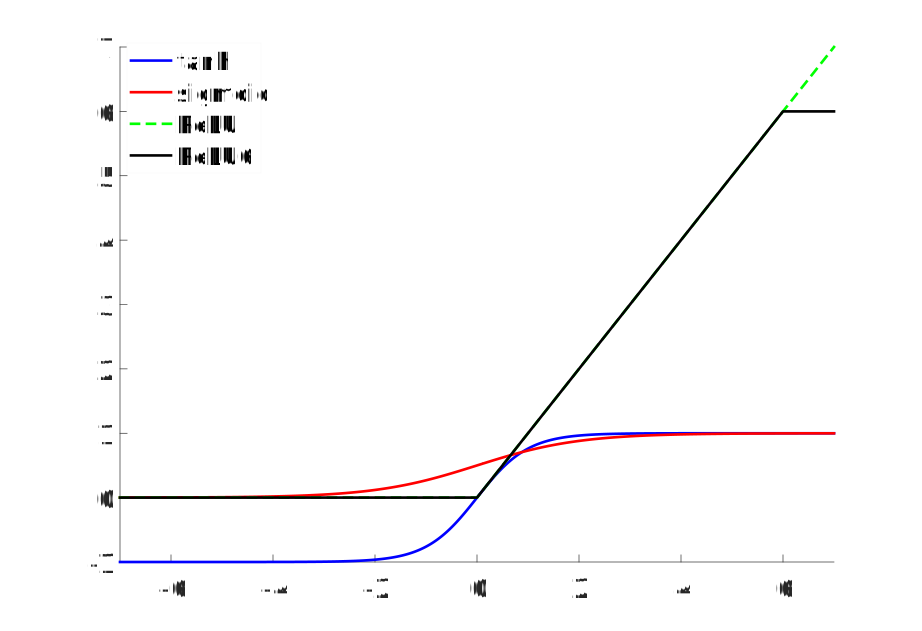
\includegraphics[width=\textwidth]{actifun.pdf}
    \caption{Activation functions}
    \label{fig:acti}
\end{figure}
%
\subsubsection{Sigmoid and Hyperbolic Tangent (Tanh)}
$Sigmoid$ and $Thanh$ are both smooth functions that can be described by equations \eqref{eq:sigmoid} and \eqref{eq:tanh}.
%
\begin{equation}
    h(x) = \frac{1}{1 + e^{-x}}
    \label{eq:sigmoid}
\end{equation}
%
\begin{equation}
    h(x) = \frac{e^{x} - e^{-x}}{e^{x} + e^{-x}}
    \label{eq:tanh}
\end{equation}
%
The two activation functions can be seen in Figure \ref{fig:acti}. They both \textquote{squeeze} the domain $\mathbb{R}$ into a smaller range, $[0, 1]$ for $Sigmoid$, and $[-1, 1]$ for the $Tanh$. However, they also saturate at the asymptotes, which means that often their gradient is close to 0. As the back-propagation algorithm requires gradient multiplication, gradient far away from the output vanishes (close to 0) and deep models do not learn: it is the \textbf{vanishing gradient problem} \cite{goodfellow_deep_2016}.
%
\subsubsection{ReLU}
To solve the problem of saturation, the Rectified Linear Unit (ReLU) has been introduced by \textcite{krizhevsky_imagenet_2012}. Equation \eqref{eq:relu} describes its behavior.
\begin{equation}
    h(x) = max(0, x)
    \label{eq:relu}
\end{equation}
%
This activation function allows faster learning, efficient gradient propagation (no vanishing or exploding gradient), and a faster computation than $Thanh$ or $Sigmoid$. However, it suffers from the \textbf{dying neuron problem} which decreases the model capacity. Some neurons become inactive (output only 0) for essentially all inputs and they \textquote{die}. A neuron that only outputs zero can be discarded. A solution would be to modify the ReLU like leaky ReLU \cite{maas_rectier_2014}, etc.

Other works try to modify the ReLU for implementation on embedded platforms. For example, \cite{howard_mobilenets_2017} uses ReLU6 (equation \eqref{eq:relu6}), which we can see in Figure \ref{fig:acti}. It is designed for fixed-point operations and quantization approaches, instead of floating-point operations which are less efficient in terms of hardware utilization and power consumption (especially on \acrshort{fpga}) \cite{david_hardware_2007}. More information about quantification can be found in Section \ref{subsec:mdopti}. Therefore, if the output $\in [ 0, 6 ]$, the number of bits for the integer part can be limited to 3 bits. We can thus increase the accuracy of the model by assigning the other bits to the decimal part.
%
\begin{equation}
    h(x) = max(0, x, 6)
    \label{eq:relu6}
\end{equation}

%
\subsection{Fully Connected layer} \label{subs:fcl}
The perceptron of Section \ref{subs:perceptron} can be considered as a linear classifier for which the decision boundary is the hyperplane, as seen in equation \eqref{eq:linearclassifer}.
%
\begin{equation}
    b + w_1 \cdot x_1 + ... + w_{n_{in}} \cdot x_{n_{in}} = 0
    \label{eq:linearclassifer}
\end{equation}
%
We can understand why the perceptron is limited because it has only a linear decision boundary. For example, we can implement the AND and OR Boolean functions using a perceptron, but it is impossible to learn the XOR function. To have a non-linear model, we must use a topology of perceptrons. This topology is composed of layers of perceptrons, where each layer, in the case of a \acrshort{cnn}, is called a \textbf{fully-connected layer}. We can see an example in Figure \ref{fig:fcn}.
%
\begin{figure}
    \centering
    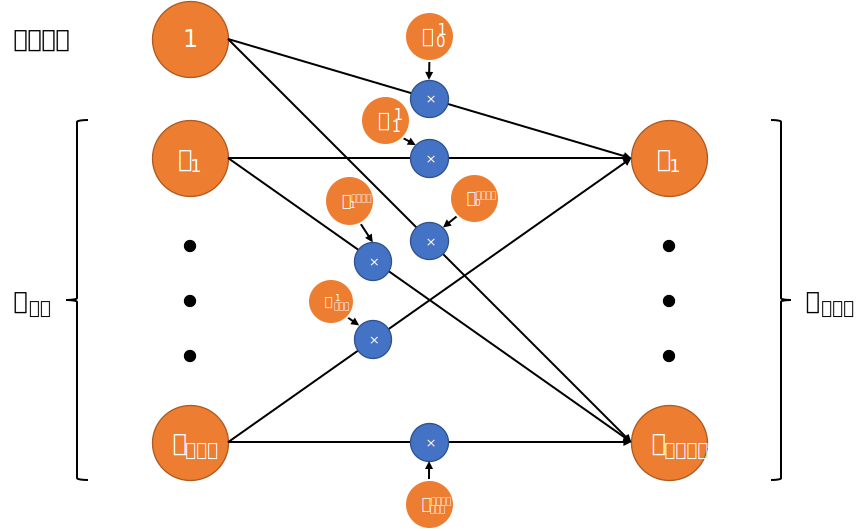
\includegraphics[width=\textwidth]{fcl.pdf}
    \caption{A fully connected layer}
    \label{fig:fcn}
\end{figure}

In the fully-connected layer, each neuron is connected to all the inputs or neurons of previous layers (as the name suggests). As the fully-connected layers are best to make a non-linear classification, we can feed those layers with extracted features, converted as a one-dimension vector \cite{khan_survey_2020}. As a result, usually, the fully-connected layers are placed at the end of \acrshort{cnn}s, where the first layers extract features from the input.

A fully-connected layer is characterized by the number of neurons, activation functions, and the values of weights. The output vector $\boldsymbol{y}$ can be expressed using equation \eqref{eq:fcn}, where $\boldsymbol{x}$ is the vector of the input of the layer and $x_0 = 1$ is the bias;   $\boldsymbol{w}$ is the vector of all the weights of the layer ($w^i_*$ are the weights of the ith perceptron and $w^*_0$ are the biases); $h$ is the activation function of the layer.
%
\begin{equation}
    \boldsymbol{y} = h(\boldsymbol{w}^T \boldsymbol{x}) \qquad \Leftrightarrow \qquad \forall o \in \{ 1, ..., N_{out} \} : y_o = h(\sum^{N_{in}}_{i=0} w^o_i \cdot x_i)
    \label{eq:fcn}
\end{equation}
%
As we have seen that perceptrons can be used to construct a non-linear classifier, we see in the next section \ref{subs:2dconv} the main operation in the \acrshort{cnn}: the \textbf{convolution}, which extracts the feature from input images.

%
\subsection{Convolution layer} \label{subs:2dconv}
A convolutional layer carries out the feature extraction process by applying a set of 3D-convolution filters to a set of input volumes, also called input \acrfull{fm}s. In an \acrshort{cnn}, the first convolutional layers extract low-level features while the deepest one extract more high-level features. The input \acrfull{fm}s are characterized by 3 parameters: \textbf{$N_{ix}$} the width; \textbf{$N_{iy}$} the height; \textbf{$N_{if}$} the depth. An illustration is in figure \ref{fig:notation:ifm}.
The input \acrshort{fm} are then processed with a kernel (of size $N_{kx} \times N_{ky} \times N_{if} \times N_{of}$), that we can see on figure \ref{fig:notation:k}) to obtain the output \acrshort{fm}s. The output \acrshort{fm}s are also characterized by its width $N_{ox}$, its height $N_{oy}$ and its depth $N_{of}$. We can also see a general output \acrshort{fm}s on figure \ref{fig:notation:ofm}.
%
\begin{figure}
    \centering
    %
    \begin{subfigure}{.32\textwidth}
    \centering
    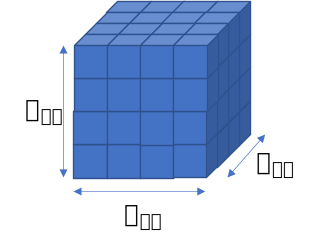
\includegraphics[width=\linewidth]{notifm.pdf}
    \caption{kernel-wise pruning}
    \label{fig:notation:ifm}
    \end{subfigure}
    %
    \begin{subfigure}{.32\textwidth}
    \centering
    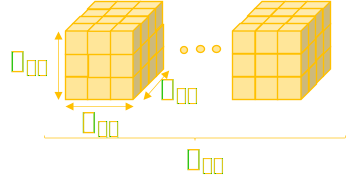
\includegraphics[width=\linewidth]{notk.pdf}
    \caption{Convolution kernel}
    \label{fig:notation:k}
    \end{subfigure}
    %
    \begin{subfigure}{.32\textwidth}
    \centering
    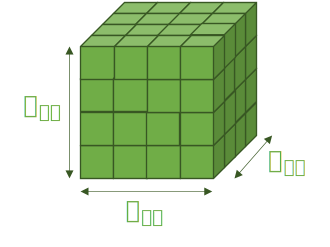
\includegraphics[width=\linewidth]{notofm.pdf}
    \caption{Output \acrshort{fm}s}
    \label{fig:notation:ofm}
    \end{subfigure}
    %
    \caption{Volumes involved in the convolution operations}
    \label{fig:notconv}
\end{figure}

The convolution operation happens as follow. We have an input \acrshort{fm} and a kernel. The kernel acts as a sliding window on the input \acrshort{fm}s. We extract a chunk of pixels of the same size of the kernel in the input \acrshort{fm}. Therefore, we perform a element-wise multiplication with the chunk of data and the kernel to obtain a pixel ouf output. Sliding this kernel on the input \acrshort{fm}s will produce an ouput \acrshort{fm}, where the output pixel at postion $(x, y)$ corresponds to the movement of the sliding window. Since one kernel produces one output \acrshort{fm}, having $N_{of}$ kernels produces then $N_{of}$ output \acrshort{fm}. An illustration of the convolution operation is in figure \ref{}.

Except for $1 \times 1$ kernels, the sliding window can not cover all input pixels and then there is a spatial reduction between the input and output \acrshort{fm}s, while there is an increase in the number of channel. However, we can keep the same dimensions using \textit{padding} on the boundary (for example adding 0).

Moreover, each time the sliding window performs a convolution, it shifts in the input \acrshort{fm}. The amount by which the filter shifts is called the \textit{stride} and it is initialy set to 1. This way we can even more reduce the width and the height of the output \acrshort{fm}s. For example, if we use padding and a stride of 2, $\frac{N_{ix}}{N_{ox}} = \frac{N_{iy}}{N_{oy}} = \frac{1}{2}$ and we use 4 times less pixels.

Finally, we can express the convolution operations mathemalically as in equation \eqref{eq:conv}.
    \begin{multline}
        \forall ox \in \{ 1, ..., N_{ox} \}, oy \in \{ 1, ..., N_{oy} \}, of \in \{ 1, ..., N_{of} \} : \\
        FM_O[ox, oy, oc] = \sum^{N_{if}}_{if=1}
        \sum^{N_{kx}}_{kx=1}
        \sum^{N_{ky}}_{ky=1}
        FM_I[ox \cdot S + kx - \lfloor \frac{N_{kx}}{2} \rfloor,  oy \cdot S + ky - \lfloor \frac{N_{ky}}{2} \rfloor, if] \cdot
        W^{of}_{if}[kx, ky]
        \label{eq:conv}
    \end{multline}

If we compare the convolutional layer with the fully-connected layer, the convolutional layer allows weight sharing and then it needs less weights. For example in AlexNet \cite{krizhevsky_imagenet_2012}, 94\% of the weights are used in the fully-connected layers. But as said earlier, 90\% of the arithmetic operations are done in the convolutional layer.

%
\subsection{Depthwise Separable Convolution}  \label{subs:dsc}
\acrfull{dsc} was first introduced by \textcite{sifre_ecole_2014}. According to \textcite{chollet_xception_2017}, \textquote{\textit{A depthwise separable convolution consists in a \textbf{depthwise convolution}, i.e. a spatial convolution performed independently over each channel of an input, followed by a \textbf{pointwise convolution}, i.e. a $1 \times 1$ convolution, projecting the channel's output by the depthwise convolution onto a new channel space}}.

It means that the \acrshort{dsc} is composed of a depthwise convolution followed by a pointwise convolution as illustrated in Figure \ref{fig:dsc}. This alternative form of convolution has been developed to reduce efficiently the arithmetic complexity, in exchange of a limited loss of accuracy \cite{liu_fpga-based_2019}. As a result, the \acrshort{dsc} has significantly fewer parameters and operations with respect to the standard convolution. Equations \eqref{eq:descopred} and \eqref{eq:descwgred} are used to calculate the reduction factors on weigths and on operations respectively, where $F_{*}$ are the factors of reduction, $W_{sc}$ and $O_{sc}$ are the weights and operations required for a standard convolution, and $W_{dsc}$ and $O_{dsc}$ are the weights and operations required for a \acrshort{dsc} \cite{liu_fpga-based_2019}.
%
\begin{equation}
    F_w = \frac{W_{dsc}}{W_{sc}} =
    \frac{N_{kx} \times N_{ky} \times N_{if} + N_{if} \times N_{of}}{N_{kx} \times N_{ky} \times N_{if} \times N_{of}} =
    \frac{1}{N_{of}} + \frac{1}{N_{kx} \times N_{ky}}
    \label{eq:descopred}
\end{equation}
\begin{equation}
    \begin{split}
        F_o &= \frac{O_{dsc}}{O_{sc}} = \frac{N_{kx} \times N_{ky} \times N_{if} \times N_{ox} \times N_{oy} + N_{if} \times N_{of} \times N_{ox} \times N_{oy}}{N_{kx} \times N_{ky} \times N_{if} \times N_{of} \times N_{ox} \times N_{oy}} \\
        &= \frac{1}{N_{of}} + \frac{1}{N_{kx} \times N_{ky}}
    \end{split}
    \label{eq:descwgred}
\end{equation}

Using equation \eqref{eq:descopred} and equation \eqref{eq:descwgred} and $3 \times 3$ kernels, the reduction of computation and parameters in comparison with the standard convolution is about 9 times \cite{zhang_channel_2019}.
%
\begin{figure}
    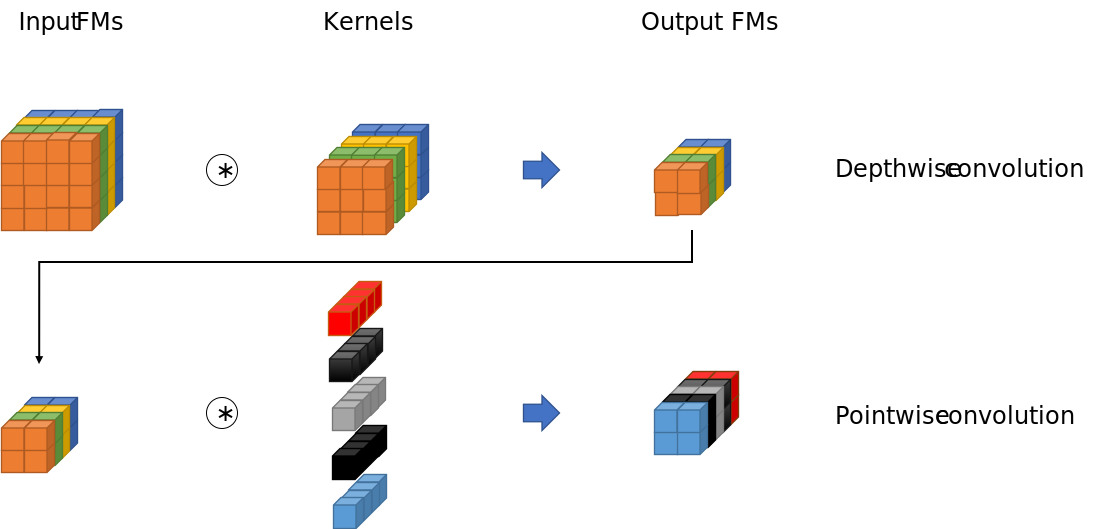
\includegraphics[width=\textwidth]{dsc.pdf}
    \caption{Depthwise Separable Convolution}
    \label{fig:dsc}
\end{figure}

%
\subsection{Pooling} \label{subs:pooling}
Pooling layers are inserted between successive convolutional layer. It aims at reducing the spatial size of each \acrshort{fm}. It reduces the number of parameters and the computation of the network while also increasing the receptive field \cite{shawahna_fpga-based_2019}. The layer divides each \acrshort{fm} in regions of size $K \title K$ and outputs one pixel from each region. This way, we can keep the number of channel and reduce each spatial dimension by $K$.

Various pooling functions can be used, but the most common form is with filters of size $2 \times 2$ where the MAX or AVG operation selects the highest pixel from 4 samples (meaning a reducion 75\%) \cite{suda_throughput-optimized_2016}. An illustration can be found in figure \ref{fig:pool}.
%
\begin{figure}
    \centering
    \includegraphics[width=\textwidth]{pooling.pdf}
    \caption{An example of pooling layers}
    \label{fig:pool}
\end{figure}

%
\subsubsection{Summary}
%
The summary of this section is provided by Figure \ref{fig:layer:summary}. An input image is transmitted to the \acrshort{cnn} then, three different kinds of layers can be used:
%
\begin{enumerate}
    \item The convolutional layer which extract the features from the input.
    \item The pooling layer which summarizes the output of the previous layer.
    \item The fully connected layer which is a non linear classifier.
\end{enumerate}
%
A typical \acrshort{cnn} is composed of two parts, which are built from stacking the previously mentioned layers \cite{matteucci_artificial_2019}:
\begin{enumerate}
    \item The feature extractor part, composed of blocks made of convolutional, activation, and pooling layers.
    \item The classifier part, composed only of fully connected layers.
\end{enumerate}
%
\begin{figure}[H]
    \centering
    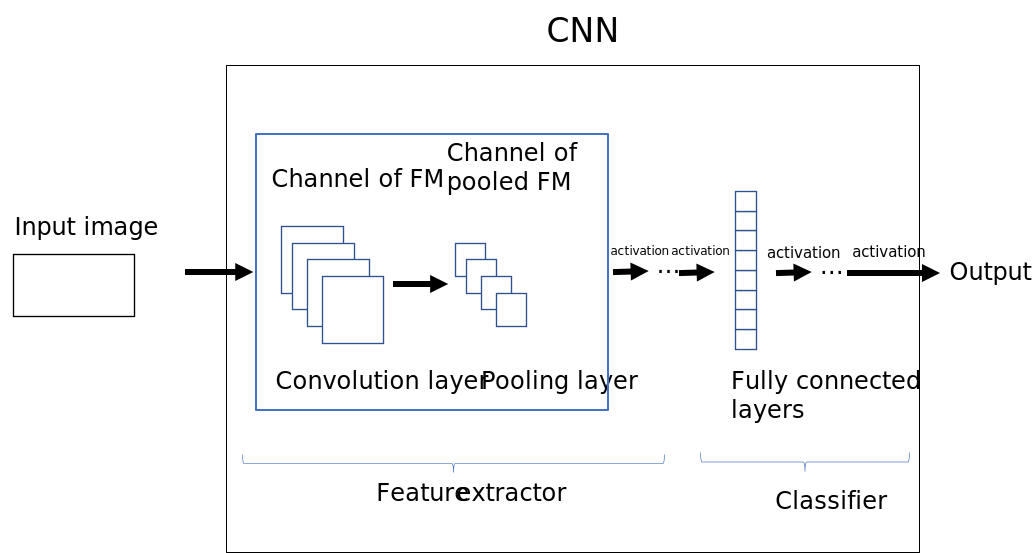
\includegraphics[width=\textwidth]{cnn_summary.pdf}
    \caption{Working principle of a CNN and the different layers which composing it}
    \label{fig:layer:summary}
\end{figure}
%
\subsection{CNN Models} \label{subsec:models}
After the analysis of the CNN structure in Section \ref{subsec:layer}, this section details some of the well-known \acrshort{cnn} networks. They are examples of how to construct an efficient \acrshort{cnn}.

%
\subsection{AlexNet}
AlexNet is a \acrshort{cnn} developed in 2012 by \textcite{krizhevsky_imagenet_2012}. AlexNet has made a breakthrough in the deep \acrshort{cnn} field and this model has won the ImageNet competition. It is made of 5 convolutional layers and 3 fully-connected layers. We can see the network in Figure \ref{fig:alexnet}. Each convolutional layer has a ReLU activation function and it uses pooling.
%
\begin{figure}
    \centering
    \includegraphics[width=\textwidth]{alexnet.pdf}
    \caption{An illustration of the architecture of AlexNet \cite{krizhevsky_imagenet_2012}}
    \label{fig:alexnet}
\end{figure}
%
\subsection{VGG}
After the success of AlexNet, research has been made to have a network with the same accuracy but lower computational complexity. VGG has been introduced by \textcite{simonyan_very_2015} in 2014, which is a deeper variant of AlexNet. It consists of 5 groups of convolutional layers, where the number of layers depends on the version of VGG. It has won the localization and the second-place tracks in the ImageNet challenge in 2014. An illustration can be found in Figure \ref{fig:vgg}. This depth has been possible by using very small ($3 \times 3$) convolution kernels: it allows a larger receptive field while having fewer parameters and more non-linearities than a larger kernel. However, it has a high memory request. We need 100MB per image to be stored in all \acrshort{fm}s for the forward propagation
%
\begin{figure}
    \centering
    \includegraphics[width=\textwidth]{VGG.pdf}
    \caption{An illustration of the architecture of VGG16 \cite{simonyan_very_2015}}
    \label{fig:vgg}
\end{figure}
%
\subsection{ResNet}
Resnet is a very deep network (between 50 and 1000 convolutional layers) proposed by \textcite{he_deep_2015} with more irregular and complex structures compared to the previous networks. \textcite{he_deep_2015} have shown that an increase of the depth does not mean an improvement in the performance of the network and this is not due to overfitting. It is because deeper models are harder to optimize than shallower ones (vanishing gradient). But intuitively, the deeper networks should have at least similar or better performance than shallower models. It is explained by the fact that we can map a deeper model into a shallower one by setting the weights to the identity.

Their solution is to add an \textquote{identify shortcut connection} that skips one or more layers to mitigate the gradient descent problem and try to set the weights to the identity. We can see the process in figure \ref{fig:resnet}. Weights between the skip connection can be used to learn a residual $F(x)$ to improve the solution. The performance of ResNet enables it to be the 2015 ILSVR winner for both localization and classification.
%
\begin{figure}
    \centering
    \includegraphics[width=0.8\textwidth]{resnet.pdf}
    \caption{ResNet building block \cite{he_deep_2015}}
    \label{fig:resnet}
\end{figure}
%
\subsection{MobileNetV2} \label{subs:mbv2}
The drive of the previous networks for accuracy has come for high computational and storage costs which are beyond the capabilities of many mobiles and embedded applications, according to \textcite{cheng_recent_2018}. For the \acrshort{cnn} training phase, it is not a problem thanks to the high performance and large disk and memory storage capacities of the \acrshort{gpu} and \acrshort{cpu} clouds. However, for the inference stage, it is difficult to deploy such networks on mobile devices such as \acrshort{fpga} because of their constraint resources:
%
\begin{itemize}
    \item The enormous computational complexity of \acrshort{cnn}s makes it difficult to deploy on real-time applications and it consumes battery power.
    \item The large number of parameters of \acrshort{cnn}s consumes considerable storage and run-time memory.
\end{itemize}

\textcite{sandler_mobilenetv2_2019} have proposed a network tailored for such constrained environments. To do so, we must first reduce the size and number of operations. They have achieved it using \acrshort{dsc}, introduced in Section \ref{subs:dsc}, and a new kind of layer: inverted residual with a linear bottleneck (observed in Figure \ref{fig:invreslinbot}). It is first composed of a $1 \times 1$ convolution to expand the number of the input \acrshort{fm} channels and then followed by a \acrshort{dsc}. The intermediate increase in the number of channels is supposed to counterbalance the loss of information that occurred by the ReLU. They have also added a skip connection to build a network of great depth, and the last convolution has a linear activation function.
%
\begin{figure}
    \centering
    \includegraphics[width=\textwidth]{mbnv2.pdf}
    \caption{inverted residual with linear bottleneck \cite{sandler_mobilenetv2_2019}}
    \label{fig:invreslinbot}
\end{figure}

%
%
\subsection{Training} \label{subsec:train}
In previous section were described the common building blocks present in \acrshort{cnn} and how to design a \acrshort{cnn}. This section aims at detailing how a network improves automatically its performance for a specific task. This is called \textit{learning}.

The learning phase starts after designing the network. However, before the model can learn, we have to initialize the weights. The most common initialization is random Gaussian distribution \cite{he_delving_2015}. However, the learning phase is affected by the initial values of the weights. If it is too small the network does not learn or if it is too large it might take a very long time to converge. Different initializations were suggested to improve the learning phase: Xavier initialization \cite{glorot_understanding_2010} and He initialization \cite{he_delving_2015}.

When values are assigned to the weights, the backpropagation algorithm can be performed in order to improve the efficiency of the network. The backpropagation algorithm is composed of two steps: the forward pass and the backpropagation. In the following sections we briefly review each of them.
%
\subsection{Forward-propagation} \label{subs:trainforward}
We use the training data as input for the model and we propagate each input through the network using the current weights. The forward propagation produces a vector of output that we can compare with the label of the input (target). This comparison is made with a loss function (for example the mean-square error, that we can see in equation \eqref{eq:mse}). To improve the accuracy of the model, we have to minimize the loss function by finding the optimal weights. This can be done using the algorithms found in the next section \ref{subs:trainbackward}. Moreover, once the model is trained, the inference consists only of the forward propagation.
%
\begin{equation}
    L(\boldsymbol{w}, \boldsymbol{w}) = \sum^{N}_{i=1} (label_i - p(x_i, \boldsymbol{w}))
    \label{eq:mse}
\end{equation}

%
\subsection{Back-propagation} \label{subs:trainbackward}
According to \textcite{ruder_overview_2017}, gradient descent optimization algorithms are the most common one used  to perform optimizations on \acrshort{nn}. These algorithms derive from the idea of gradient descent. As said in the previous section, gradient descent is a way to minimize the loss function in order to parametriz the parameters of the model (weight). Equation \eqref{eq:gd} defines the gradient descent algorithm, where $\eta$ is the learning rate, a positive scalar determining the size of the step in the direction minimizing the gradient \cite{ruder_overview_2017, goodfellow_deep_2016}. If we update the weight in the opposite direction of the gradient, we can reach a local minimum.
%
\begin{equation}
    \boldsymbol{w} = \boldsymbol{w} - \eta \frac{ \partial L( \boldsymbol{x}, \boldsymbol{w} ) }{\partial \boldsymbol{w}}
    \label{eq:gd}
\end{equation}

\textbf{The original gradient descent} or \textbf{batch gradient descent} computes the gradient using the whole dataset (the batch) \cite{ruder_overview_2017, matteucci_artificial_2019}. Equation \eqref{eq:gd-grad} is used to compute this batch gradient. However, this might be impossible to do in practice if the dataset is too large. Indeed, Indeed, the gradient of the whole dataset has to be computed for each update. Therefore, variations of this algorithm have been proposed to make the gradient descent practical.
%
\begin{equation}
    \frac{ \partial L( \boldsymbol{x}, \boldsymbol{w} ) }{\partial \boldsymbol{w}} = \frac{1}{N_{in}} \sum^{Nin}_{i = 0} \frac{ \partial L( x_i, \boldsymbol{w} ) }{\partial \boldsymbol{w}}
    \label{eq:gd-grad}
\end{equation}

\textbf{Stochastic gradient descent}, instead of using the entire dataset, performs the gradient descent algorithm on each training sample of the whole dataset \cite{ruder_overview_2017, matteucci_artificial_2019}. Equation \eqref{eq:sgd-grad} computes the stochastic gradient descent. It avoids the redundant computation of the batch gradient descent. It learns faster and can reach better local minima, however, it is complicated to find the global minimum.
%
\begin{equation}
    \frac{ \partial L( \boldsymbol{x}, \boldsymbol{w} ) }{\partial \boldsymbol{w}} = \frac{ \partial L( x_i, \boldsymbol{w} ) }{\partial \boldsymbol{w}}
    \label{eq:sgd-grad}
\end{equation}

\textbf{Mini-batch gradient descent} is a trade-off between the two previous approaches \cite{ruder_overview_2017, matteucci_artificial_2019}. It performs an update of the weights for every mini-batch of the whole dataset. Equation \eqref{eq:bgd-grad} computes the mini-batch gradient descent, where $N$ is the number of training samples. It shows a better convergence than stochastic gradient descent by reducing the variance and has less computations than batch gradient descent.
%
\begin{equation}
    \frac{ \partial L( \boldsymbol{x}, \boldsymbol{w} ) }{\partial \boldsymbol{w}} = \frac{1}{N} \sum^{N < N_{in}}_{i = 0} \frac{ \partial L( x_i, \boldsymbol{w} ) }{\partial \boldsymbol{w}}
    \label{eq:bgd-grad}
\end{equation}

%
%
